\subsubsection{Biological testing\label{sec:bio1}}

The eight triazoles made in \ref{sec:Tris} (see \ref{fgr:finals_1}) were tested for antibacterial and anti-biofilm activity. 

\begin{figure}[H]
	\begin{center}
		\schemeref[HL2T4Cip]{cmpd:HL2T4Cip}
		\schemeref[HL4T4Cip]{cmpd:HL4T4Cip}
		\schemeref[HL6T4Cip]{cmpd:HL6T4Cip}
		\schemeref[6HHQT4Cip]{cmpd:6HHQT4Cip}
		\schemeref[HL4T4Tri]{cmpd:HL4T4Tri}
		\schemeref[HL6T4Tri]{cmpd:HL6T4Tri}
		\schemeref[6HHQT4Tri]{cmpd:6HHQT4Tri}
		\schemeref[PQST4Tri]{cmpd:PQST4Tri}	
		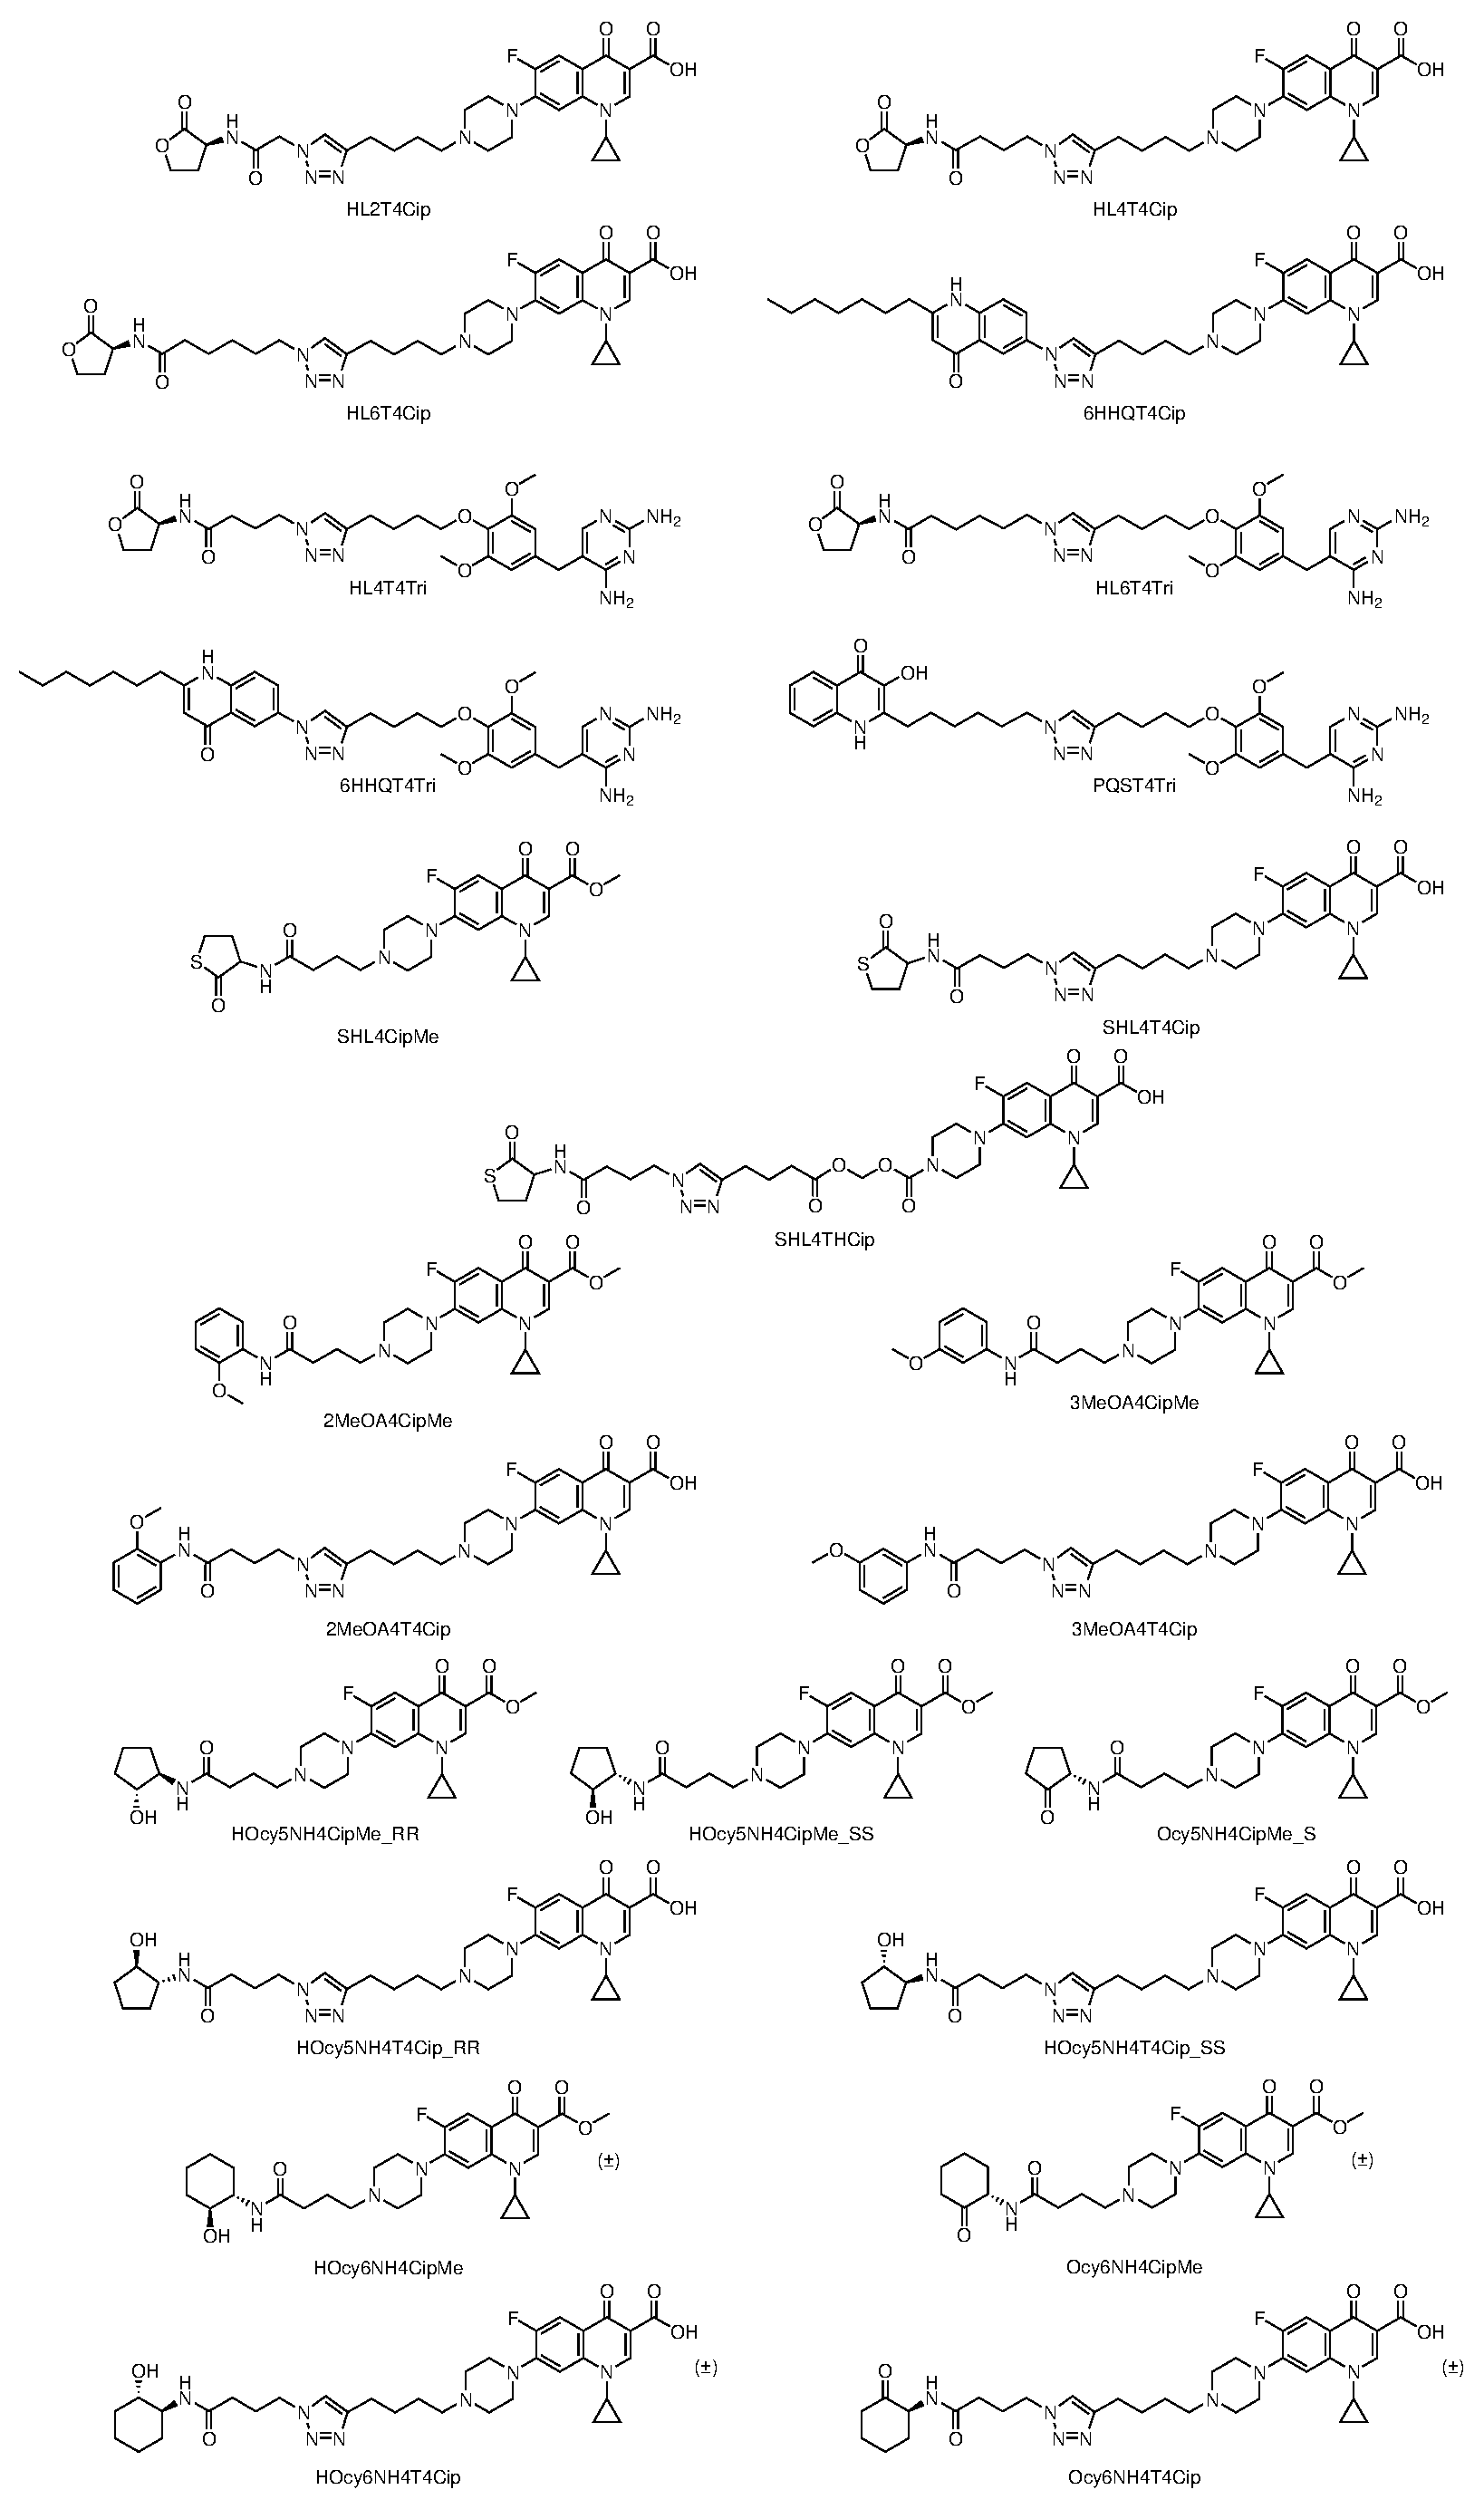
\includegraphics[width=\textwidth]{finals_1}
		\caption{
 		\label{fgr:finals_1}}
	\end{center}
\end{figure}

The compounds were tested in PAO1, and YM64 which is missing 4 main efflux pumps.
Antibacterial activity was measured by measurement of turbidity at 595 nm at 5 h and 24 h.
The compounds were tested at 6 concentrations between 2 and 0.0625 $\mu$M in LB in 96-well plates.
In YM64 at 5 h the HSL-ciprofloxacin conjugates \compound{cmpd:HL2T4Cip}, \compound{cmpd:HL4T4Cip} and \compound{cmpd:HL6T4Cip} showed slight activity at the highest concentration, but not as high as ciprofloxacin \compound{cmpd:Cip}.
This activity was not visible by 24 h and the compounds had no effect on biofilm formation (data not shown).
HL4, HHQ and PQS were also tested as controls, but had little effect on bacterial or biofilm growth (data not shown).

\begin{figure}[H]
	\begin{center}
		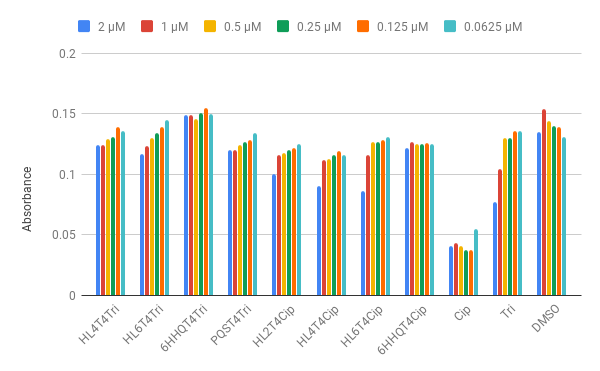
\includegraphics[width=\textwidth]{YM64_5h}
		\caption{YM64 5 h.\label{fgr:YM64_5h}}
	\end{center}
\end{figure}

In PAO1 \compound{cmpd:HL6T4Cip} showed similar activity to ciprofloxacin \compound{cmpd:Cip} at the highest concentration (see \ref{fgr:PAO1_5h})

\begin{figure}[H]
	\begin{center}
		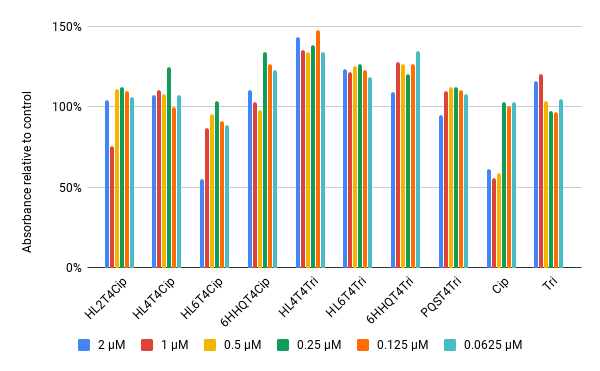
\includegraphics[width=\textwidth]{PAO1_5h}
		\caption{PAO1 5 h.\label{fgr:PAO1_5h}}
	\end{center}
\end{figure}


We hypothesised that the lack of biological activity was a result of the compounds being unable to dissociate from the cell wall. 





\subsubsubsection{Cleavable conjugates}

The eight cleavable HSL-ciprofloxacin conjugates, two controls and two alkynes described in \ref{sec:cleavable} (see \ref{fgr:finals_cleavable}) were tested for antibacterial and anti-biofilm activity. 

\begin{figure}[H]
	\begin{center}
		\schemeref[HL2THCip]{cmpd:HL2THCip}
		\schemeref[HL4THCip]{cmpd:HL4THCip}
		\schemeref[HL6THCip]{cmpd:HL6THCip}
		\schemeref[HL2TMeCip]{cmpd:HL2TMeCip}
		\schemeref[HL4TMeCip]{cmpd:HL4TMeCip}
		\schemeref[HL6TMeCip]{cmpd:HL6TMeCip}
		\schemeref[BnTHCip]{cmpd:BnTHCip}
		\schemeref[BnTMeCip]{cmpd:BnTMeCip}		
		\schemeref[Y4HCip]{cmpd:Y4HCip}
		\schemeref[Y4MeCip]{cmpd:Y4MeCip}
		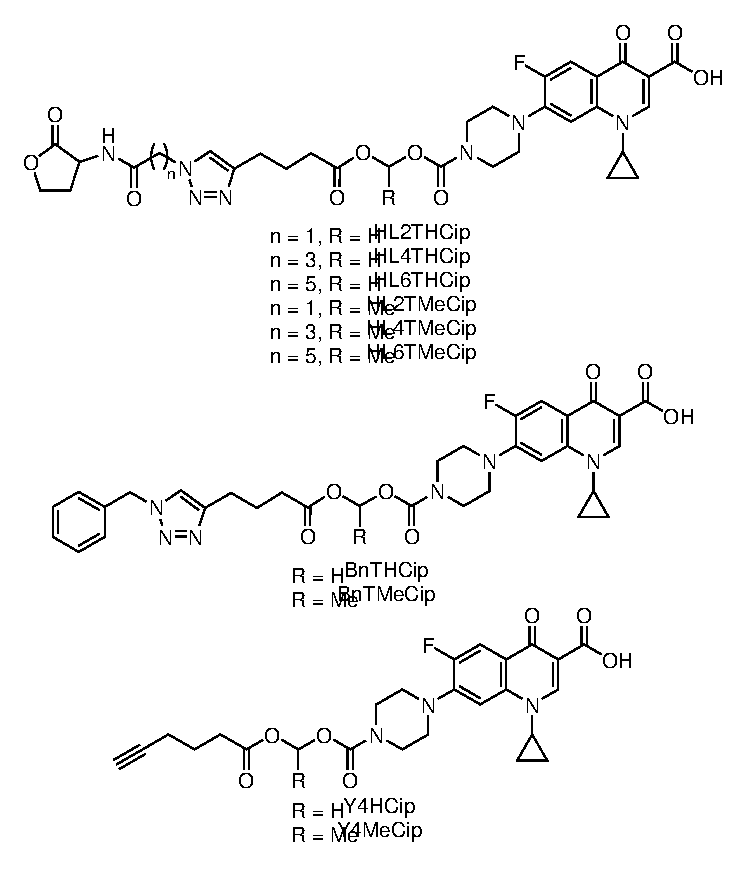
\includegraphics[scale=1]{finals_cleavable}
		\caption{
 		\label{fgr:finals_cleavable}}
	\end{center}
\end{figure}

Here there was more success, although the activity is still not as high as for ciprofloxacin \compound{cmpd:Cip}.
The compounds with methoxy linkers (R = H) showed activity at high concentrations. A longer linker seems to give higher activity. \compound{cmpd:HL4THCip} and \compound{cmpd:HL6THCip} showed activity comparable with ciprofloxacin \compound{cmpd:Cip} at high concentrations.
Unfortunately the control \compound{cmpd:BnTHCip} and alkyne \compound{cmpd:Y4HCip} showed higher activity than the conjugates, indicating that the HSL head wasn't helping the effect.
It is likely that the activities of these compounds can be explained by molecular weight and/or polarity.

The conjugates with an ethoxy linker (R = Me) did not show any activity. This suggests that they either didn't enter cells or weren't suitable substrates for esterases.
The alkyne does show some activity, indicating that maybe it can penetrate cells a more than the others as it is smaller.

\begin{figure}[H]
	\begin{center}
		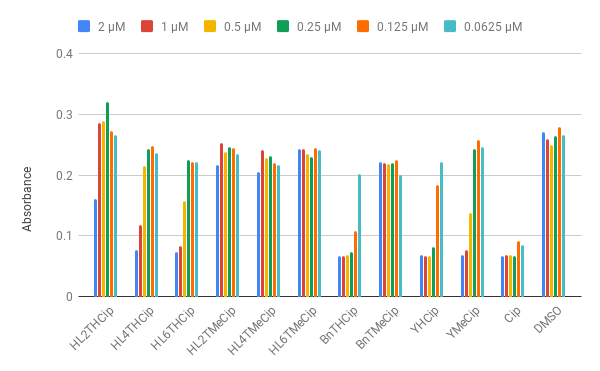
\includegraphics[width=\textwidth]{YM64_5h_cleavable}
		\caption{YM64 5 h cleavable conjugates.\label{fgr:YM64_5h_cleavable}}
	\end{center}
\end{figure}

To address this a sceond set of conjugates were prepared in collaboration with Professor Eddy Sotelo, a visiting academic in the Spring group. 

OR:

you could go with something like: in parallel with the perpetration of xxx, a second ciprofloxicin alkyne was prepared by Eddie Soleto. and do the bio together. just be more positive nad view it as a collaboration, just because yours didn't work doesnt mean they didnt contribute to the knowledge that you need the biocleavable linker. In fact. he needed you and your azides! :) 

However, initial results in YM64 (a PAO1 mutant lacking efflux pumps) show that the one compound that may show comparable results to ciprofloxacin is a control compound with a benzyl group attached. However, both compounds completely inhibited bacterial growth at all concentrations tested, so it is not clear if the compound is better than ciprofloxacin. Testing in PAO1 should be completed this week; as antibiotics are usually in this wild-type strain the difference between ciprofloxacin and the conjugate should show up without lowering the concentration. 